\section{The microscopic description of atomic systems}
Molecular dynamics, and computational statistical physics at large, aim at simulating on the computer the behavior of physical systems.
The hope is that one can infer quantities and properties of real-life interest from observing the results of numerical simulations, which may be relevant to understand the material properties of many-particle systems, or the nature of interactions in complex systems such as those found in biology.
Computational simulations can thus act as surrogate experiments in cases where experimental setups are hard to achieve, or measurements are impossible.
They can also be seen as surrogate tests of theoretical models, as they allow to test the validity of a mathematical description by comparing numerical predictions to experimental data. Molecular dynamics, in particular, is concerned with simulating atomic systems, most often (and as we shall systematically do) using a classical description.


We consider a system of $N$ particles evolving in $d$-dimensional space. The classical description contends that the \textit{state} of a system is the datum of the positions and momenta of every particle in the system. We can interpret this as the statement that, given full knowledge of the positions and momenta at some initial time, and of the forces at play, one can deduce exactly the positions and momenta at any future time.

\begin{definition}[Phase space]

    We describe the positions and momenta of the atoms as vectors
    $$ q=(q_{1,1},\dots,q_{1,d},\dots ,q_{N,1},\dots,q_{N,d})^\intercal \in \R^{dN},$$
    $$ p=(p_{1,1},\dots,p_{1,d},\dots ,p_{N,1},\dots,p_{N,d})^\intercal \in \R^{dN},$$

    where $q_i \defeq (q_{i,1},\dots, q_{i,d})^\intercal$ is the position vector of the $i$-th particle, and similarly for $p$. 
    In practice, it is often the case that each $q_i$ is restricted to some $d$-dimensional manifold $\cD$, called the configuration space. For our purposes, we will always take $\cD=\R^{d}$ or $\cD=(L\mathbb T)^{d}$, where $L>0$ is some size parameter. Phase space, then, is the set of possible microscopic states of the system, that is, the set
    $$\mathcal E=\cD^{N} \times \R ^{dN}$$

    Trajectories through phase space, that is functions

    $$\left\{\begin{aligned} \R_+  &\mapsto \mathcal E \\ 
                            t  &\mapsto  (p_t,q_t)\end{aligned}\right.,$$
    can be seen as describing time evolutions of the system, objects which will be central to our study.
\end{definition}

It is not clear \textit{a priori} why we should choose momenta to describe the kinetic quality of the system, rather than velocities. However it is of no importance since we can change from one description to the other via the relation
$$v=M^{-1}p,$$
where $M\in \R^{dN \times dN}$ is a diagonal matrix recording the masses of each particle ($d$ times per particle), and $v$ is the velocity vector.


In order to describe the evolution of the system's state, one must specify a dynamical law. This is done by giving a function

\begin{equation*}
    \left\{ \begin{aligned} \cD &\mapsto \R \\
                            q &\mapsto V(q) \end{aligned} \right. ,
\end{equation*}

$V$ whose gradient in the $i$-th particle's coordinates 
$$ \nabla_{q_i} V \defeq (\partial_{q_{i,d}},\dots , \partial_{q_{i,d}})^\intercal $$
gives minus the force vector acting on the $i$-th particle. In the case where $\cD = (L\mathbb T)^{dN}$, it will be convenient to think of $V$ as a function from $\R^{dN}$ to $\R$ which is $C^1$ and $L$-periodic in each direction.

$V$ is called the potential, and, as it encodes the dynamics of the system, it is of paramount importance. The time evolution of the system, then, is described by Newton's second law:

$$\frac{\text{d} p}{\dt}=-\nabla V(q)$$.

It will be convenient for our analysis to use of reformulation of Newton's equations, based on the Hamiltonian of a system.

\begin{definition}[Hamiltonian]
    The Hamiltonian of a classical system is its total energy, which is the sum of a kinetic energy term depending only on the momenta and a potential energy term depending only on the positions.

    \begin{equation}
        H(q,p)=\frac12p^\intercal M^{-1}p+V(q)
    \end{equation}
\end{definition}

Using the Hamiltonian, we can rewrite the classical equations of motion as

\begin{equation}
\label{Hamiltonian dynamics}
\begin{cases}
    \text d q_t=M^{-1}p_t\dt=\nabla_p H(q_t,p_t)\dt\\
    \text d p_t=-\nabla V(q_t)\dt=-\nabla_q H(q_t,p_t)\dt
\end{cases},
\end{equation}

The potential is the most important part of the microscopic description, and accordingly, the main problem in establishing a physical model of this kind is to determine potential functions which adequately capture the dynamic behavior of a given system. 
The choice of a classical description automatically implies a degree of approximation, since behavior arising from the laws of quantum mechanics, which may be relevant at a microscopic level, are described by Newton's law.
 Furthermore, if the aim is to simulate such systems numerically, computational constraints imply that some compromise has to be reached between theoretical accuracy and computational cost. 
 If, for small systems, it may be possible to simulate all atomic interactions, for larger or more complex systems, it is often to use potential functions which are both cheap from a computational point of view and empirically shown to be accurate enough for the purpose of a simulation.
 
 Our main numerical example will be the system given by the following potential, which is of this empirical form, and which is often used to describe the microscopic behavior of chemically inert fluids, such as Argon.

 \begin{example}[The Lennard-Jones fluid]
    We fix $L>0$, $d=3$, and $N$ the number of particles. The Lennard-Jones fluid is the classical system given by the potential

    \begin{equation}
        \label{Lennard-Jones potential}
        V_{\mathrm{LJ}}(q)=\sum_{i=1}^N\sum_{j<i} 4\varepsilon \left( \left(\frac{|q_i-q_j|}{\sigma}\right)^{-12} - \left(\frac{|q_i-q_j|}{\sigma}\right)^{-6} \right).        
    \end{equation}
     
    Note that $V_{\mathrm{LJ}}$ is given by a sum over pairs of particles,

    $$V_{\mathrm{LJ}}(q)=\sum_{1\leq i < j \leq N} v(|q_i-q_j|),$$

    where $v$ is a radial function

    $$v(r)=4\varepsilon \left( \left( \frac{\sigma}{r}\right)^{12}-\left(\frac{\sigma}{r} \right)^6\right).$$

    $\varepsilon$, an energy, and $\sigma$, a length, are shape parameters which respectively control the depth of the potential well of $v$ and the equilibrium distance $2^{1/6}\sigma$.
    As seen on Figure \ref{fig:lennard_jones}, the potential combines two effects. At small interparticular distances, the dominant term is in $r^{-12}$, which translates into a strongly repulsive force between close pairs of particles, and makes individual particles essentially impenetrable.
    At long range, the dominant term is in $-r^6$, which translates into a weakly attractive force between distant particles. Contrary to the repulsive term, which is empirical, this scaling has a theoretical origin in the Van der Waals forces.
    From a computational standpoint, the fact that $v$ is an even function of $r$ allows one to compute the normalized force while sparing the expense of computing a square root, while the identity $r^{12}=(r^6)^2$ allows further economy.
    The shape parameters $\sigma$ and $\varepsilon$ must be chosen empirically to describe the behavior of a particular atomic species. For Argon, values of reference are: $\sigma=$ , $\varepsilon=$.
 \end{example}

 \begin{figure}[htbp]
    \begin{center}
      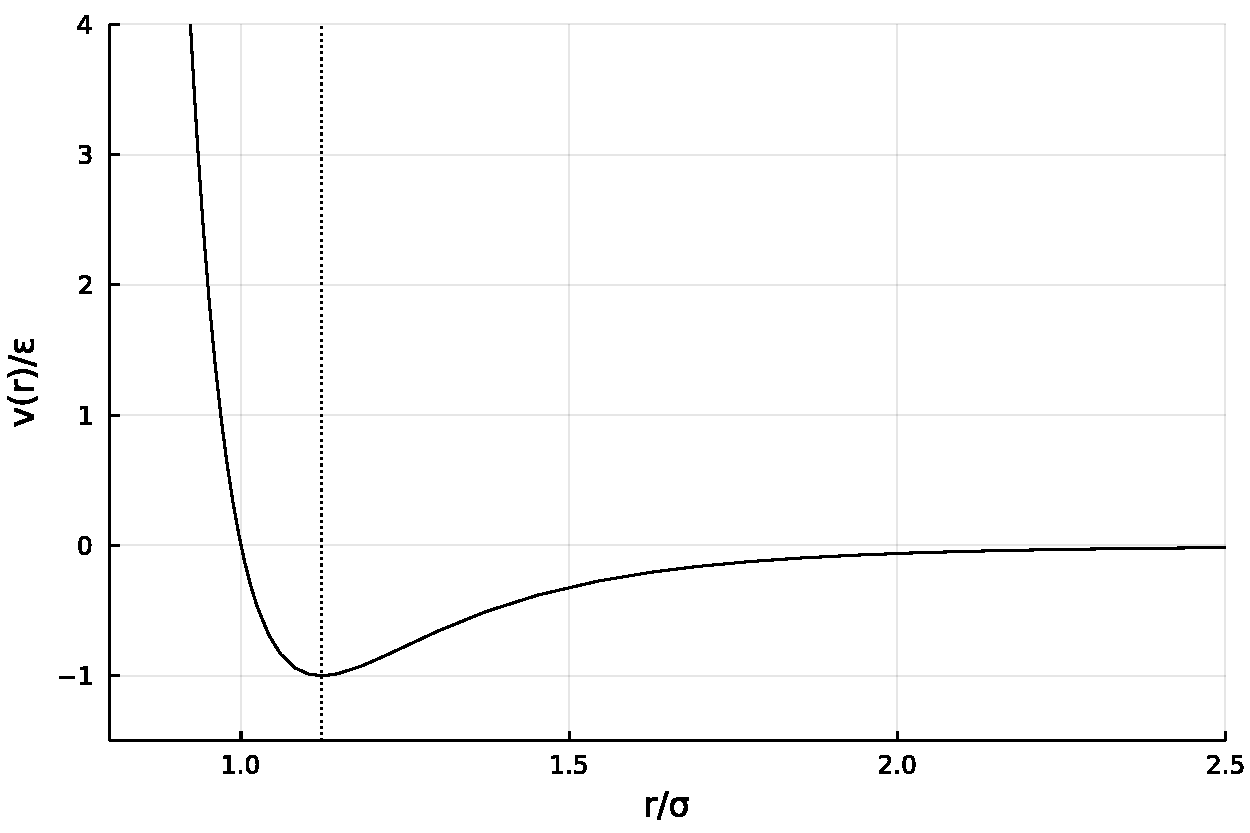
\includegraphics[width=0.7\linewidth]{figures/chapter1/lennard_jones.pdf}
      \caption{ \label{fig:lennard_jones}
        The pair potential $v$, with lengths and energy given in reduced units. The equilibrium interparticular distance is indicated by the vertical dotted line.
      }
    \end{center}
  \end{figure}

\section{Reduced units}

\section{Statistical ensembles}
The microscopic description is interesting from a theoretical standpoint, but it fails to be relevant when attempting to describe the behavior of atomic systems with a macroscopic number of particles, of the order of Avogadro's number ($6.02 \times 10^{23} $).
Besides the technical impossibility of measuring to a high accuracy the configuration of such systems, and that of recording the information required to track it (coincidentally, the total amount of digitally stored information on Earth is estimated to be $10^{23}$ bytes as of 2022), it is also the case that knowledge of a system at this level of detail is unnecessary to describe the quantities which are relevant to our macroscopic experience.
In the instance of a gas at thermal equilibrium, examples of relevant quantities are total energy, pressure, temperature, density, which, while of course resulting from the internal state of the system, are independent of the minutiae of individual atomic motions: loosely speaking, one may describe the macroscopic state of a system by only a handful of macroscopic variables, loosing track of the myriad of microscopic degrees of freedom.
An important point is that for a given macroscopic state, there are many microscopic configurations which are compatible with our observations. This motivates defining the macroscopic state of a system as a probability distribution over phase space, which we may interpret as assigning to each microscopic configuration a likelihood that this configuration underlies the macroscopic state.

This does not tell one how to choose the distribution over microscopic states. However, it seems reasonable to assign positive probabilities to states compatible with the macroscopic constraints, and in such a way as to make the weakest possible assumptions on this microscopic state, or in other words contain the least amount of information about the system, given the macroscopic constraints. The mathematical translation of this idea is given by the principle of maximal entropy. Given a class of probability distributions compatible with the macroscopic constraints, define the macroscopic state as the one which maximizes the entropy, which is defined for a probability distribution $\rho$ by

\begin{equation}
    \label{entropy}
    \mathfrak S(\rho)=-\int_{\mathcal E} \rho(x)\ln(\rho(x))\dx.
\end{equation}

The specification of a probability distribution over states is called a thermodynamic ensemble. We will be considering two ensembles:

\begin{example}[Microcanonical ensemble]

    The microcanonical ensemble is the suitable model for an isolated system in thermodynamic equilibrium, evolving under Hamiltonian dynamics. The number of particles $N$, the volume $V=L^3$, and the energy $E$ is fixed. We will alternatively refer to the microcanonical ensemble as the NVE ensemble.
     Because the constant energy condition constrains the compatible microstates to level sets of $H$, which in general will be negligible subsets of $\mathcal E$, some care must be taken in defining the microcanonical measure, since one cannot express the macroscopic constraints by a family of probability densities.
      However, under suitable assumptions on $V$, one can define the microcanonical measure as a weak limit of uniform distributions over level \textquote{shells} of $H$:
    $$\int_\mathcal{E} \varphi \text d\mu_{NVE} \defeq \underset{\varepsilon \to 0}{\mathrm{lim}} \frac{1}{|S(E,\varepsilon)|}\int_{S(E,\varepsilon)} \varphi(q,p) \text d q \text d p,$$
    where 
    $$S(E,\varepsilon) = \{ (q,p) \in \mathcal E |\ H(q,p) \in [E-\varepsilon,E+\varepsilon]\}.$$
    
    This is consistent with the fact that, for a set $A$ with finite Lebesgue measure, the probability distribution on $A$ which maximizes the entropy is the uniform distribution on $A$. 
    It is possible, using the coarea formula, to derive a precise expression for this limit, which is, however, of limited practical interest.
    
\end{example}


\begin{example}[Canonical ensemble]
    Isolated systems in thermal equilibrium are not typically those that we encounter in experiments. Instead, it is more common to observe systems which are in thermal equilibrium with respect to their environment, an ambient \textit{heat bath} at a fixed temperature.
    The total energy of such systems is not fixed: small fluctuations can occur as energy is exchanged back and forth between the heat bath and the system. However, the average energy $\bar E$ is fixed. 
    This is the macroscopic constraint that defines the canonical ensemble. For a fixed $N,V,\bar E$, define the density of the the canonical measure as the maximizer:

    $$ \underset{\rho \in \mathcal A}{\mathrm{argmax}}\ \mathfrak S(\rho)$$
    where $\mathcal A$ is the set of admissible densities
    $$\mathcal A=\{ \rho: \mathcal E \mapsto \R_+ |\ \int_{\mathcal E} \rho =1, \int_{\mathcal E} H(q,p)\rho(q,p)\text d q \text d p=E \}.$$

    Solving the Euler-Lagrange equation associated with this constrained optimization problem yields that the only admissible solution can be written under the form:

    $$ \rho^*(q,p)= \frac 1{Z} e^{-\beta H(q,p)}.$$

    Furthermore, one can show that $\rho^*$ is indeed the unique maximizer.
    Here, $-\beta$ and $1+\ln Z$ are the critical Lagrange multipliers associated respectively with the energy constraint and the normalization constraint. Thus
    $$Z=\int_{\mathcal E} e^{-\beta H(q,p)}\text d q \text d p$$
    is a normalization constant called the partition function, and $\beta$ is a tuning parameter related to the value of $\bar E$. The physical interpretation of $\beta$ is that of an inverse temperature,

    $$ \beta = \frac 1{k_B T},$$
    where $k_B=1.38 \times 10 ^{-23} \mathrm{J\cdot K^{-1}}$ is Boltzmann's constant. For obvious reasons, we prefer to refer to the canonical ensemble as the NVT ensemble (rather than the NV$\bar {\text E}$)
\end{example}

\begin{remark}
One can go further and observe that when observing a fixed volume of unconfined gas in thermal equilibrium, the total number of particles $N$ is not fixed. Instead, this fluctuates as particles are constantly exchanged with an ambient particle reservoir. Instead, the average number of particles $\bar N$ is fixed. The resulting ensemble is called the grand canonical or $\mu$VT ensemble. This, and many other constructions are possible, but we will restrict our attention to the NVE and NVT cases. 
\end{remark}

The main interest in obtaining such a description is that one can then express the macroscopic state of a system in terms of averages of microscopic observables with respect to the ensemble measure.

\section{From microscopic dynamics to macroscopic observables}

\begin{definition}[Observables]
    An observable is simply a measurable function 
    $$\varphi : \mathcal E \mapsto \R$$

\end{definition}

One can also consider vector-valued observables, such as the velocity. The potential energy $V$ (viewed as a function on $\mathcal E$), the kinetic energy $(q,p) \mapsto p^\intercal M^{-1}p/2$ and the Hamiltonian $H$ are obvious examples of observables.
Observables relate the microscopic state of the system to macroscopic quantities, through ensemble averages. Given a macroscopic system defined by an equilibrium ensemble $\mu$ and an observable $\varphi$, we are interested in computing its average over the ensemble

\begin{equation}
    \label{ensemble_averages}
\E_\mu[\varphi] \defeq \int_{\mathcal E} \varphi(q,p) \mu(\text dq,\text dp).
\end{equation}
Two problems arise. One is, for a given macroscopic quantity of interest, how to define the microscopic observable $\varphi$ which corresponds to this quantity. The second, once we have properly defined $\varphi$, is how to compute averages (\ref{ensemble_averages}). 
This second problem is one of statistically sampling a high-dimensional measure, which is a difficult problem in general. Our broad strategy, which will remain the same in the NVE and NVT case, is to define dynamical processes $(X_t)_{t\geq 0}$ on $\mathcal E$ which are invariant for the target measure $\mu$, and then consider estimates of $\E_{\mu}[\varphi]$ through the computation of ergodic averages:

\begin{equation}
\label{ergodic_averages}
 \frac{1}{T}\int_{0}^T \varphi(X_t)dt,
\end{equation}

which we may hope will converge to the target value. The convergence of ergodic averages can be shown not to hold in generality, and is something which must be proven on a case by case basis, though general criteria can be derived.
Furthermore, if the underlying dynamic is stochastic, then the variance of the random variables (\ref{ergodic_averages}) becomes an issue, which one must control.
However, empirical practice shows that ergodic averages obtained from computer simulations, even for a modest number of atoms, agrees very well with experimental data for certain types of systems, even in the absence of theoretical guarantees. We will demonstrate an example in the next chapter.